
\chapter{Análise Bibliográfica sobre Criptografia Quântica, por André Larrosa Chimpliganond}

% começou
% invadindo denovo lenovo
\section{Planejamento do estudo}
Como se transmitir informações de modo que esta só possa ser acessada pela pessoa certa? Responder essa pergunta e elaborar métodos para por a solução em prática é área de estudo da criptografia. Utilizando de alta complexidade matemática, técnicas de criptografia codificam informações de modo que só possam ser decodificadas por quem possuir a chave. Mas como o advento e evolução da computação quântica afeta a maneira como criptografamos os dados?

Partindo dessa pergunta, podemos explorar outras que irão nortear o trabalho:
\begin{itemize}
    \item Quais conceitos relacionados à esse embate entre a criptografia e computação quântica?
    \item Quais autores, instituições e nações estão à frente desse tema?
    \item Como esse conteúdo tem se desenvolvido ao longo do tempo?
\end{itemize}


\subsection{Ferramentas}
Será utilizada a interface web para o pacote Bibliometrix (Biblioshiny). Bibliometrix é um pacote R que fornece um conjunto de ferramentas para a investigação quantitativa em cientometria e bibliometria.


\section{Coleta de dados}

A coleta de dados feita usando o Web Of Science  no dia 09 de fevereiro de 2022, acessado por meio do Portal de Periódicos da CAPES.

Foram feitas buscas nas coleções \textbf{Science Citation Index Expanded (SCI-EXPANDED)--1945-presente}, \textbf{Conference Proceedings Citation Index – Science (CPCI-S)--1990-presente} e \textbf{Emerging Sources Citation Index (ESCI)--2017-presente}. 

Foi usada a seguinte \query\  de busca

\textit{\textbf{(quantum or  post-quantum) and (cryptography or cryptanalysis or encryption)}}


%\lstinputlisting[numbers=left,basicstyle=\normalsize\ttfamily,caption={\query\  de busca sobre criptografia quântica.}, label=CQA@andrelarrosacryptQuery]%label
%{experiments/andrelarrosacrypt/AnaliseBibliometrica/CriptografiaQuantica/query.txt}
%nao ta achando a query


\subsection{Explicação para os termos de busca usados}

Foram elaboradas duas cláusulas de busca unidas por \textit{and}. A primeira foca nos elementos relacionados ao universo quântico, enquanto a segunda faz referência à criptografia.

Os 10522 registros obtidos encontram-se no github do projeto, em \url{https://github.com/jhcf/Comput-Experim-20212/experiments/andrelarrosacrypt/AnaliseBibliometrica/CriptografiaQuantica/rec_1.txt} e \url{https://github.com/jhcf/Comput-Experim-20212/experiments/andrelarrosacrypt/AnaliseBibliometrica/CriptografiaQuantica/rec_2.txt}. 
% arquivo maior que  50MB

Foram exportadas todas as informações disponíveis na Web Of Science de cada documento.

\section{Análise dos dados}

\subsection{Filtragem de registros}


Após carregar o \dataset\ na plataforma biblioshiny, foi feita uma filtragem dos documentos com o intuito de selecionar apenas os artigos publicados em revistas científicas (\textit{ARTICLE}). Após a filtragem, sobraram 7131 documentos. Esse novo dataset será nomeado CriptografiaQuanticaArtigos ou CQA@andrelarrosacrypt.

\subsection{Informações principais do \dataset\   CQA@andrelarrosacrypt}
\begin{description}
    \item[Período]	1988 - 2022
    \item[Fontes]	675
    \item[Documentos]	7131
    \item[Média de anos após a publicação]	8.31
    \item[Média de citações por documento]	33.05
    \item[Média de citações por ano por documento]	2.75
    \item[Referências]	83981
    \item[Palavras-chave (Keywords Plus (ID))]   3187
    \item[Palavras-chave (Author's Keywords (DE))] 8201
    \item[Autores]   10925
    \item[Aparições de autores]	28034
    \item[Autores de documentos de autoria única]	436
    \item[Autores de documentos de autoria múltipla]	10489
    \item[Documentos de autoria única]	706
    \item[Média de documentos por autor]	0.653
    \item[Média de autores por documento]	1.53
    \item[Média de co-autores por documento]	3.93
    \item[Index de colaboração]        1.63
\end{description}


\subsection{Evolução da Produção Científica}

\begin{figure}
    \centering
    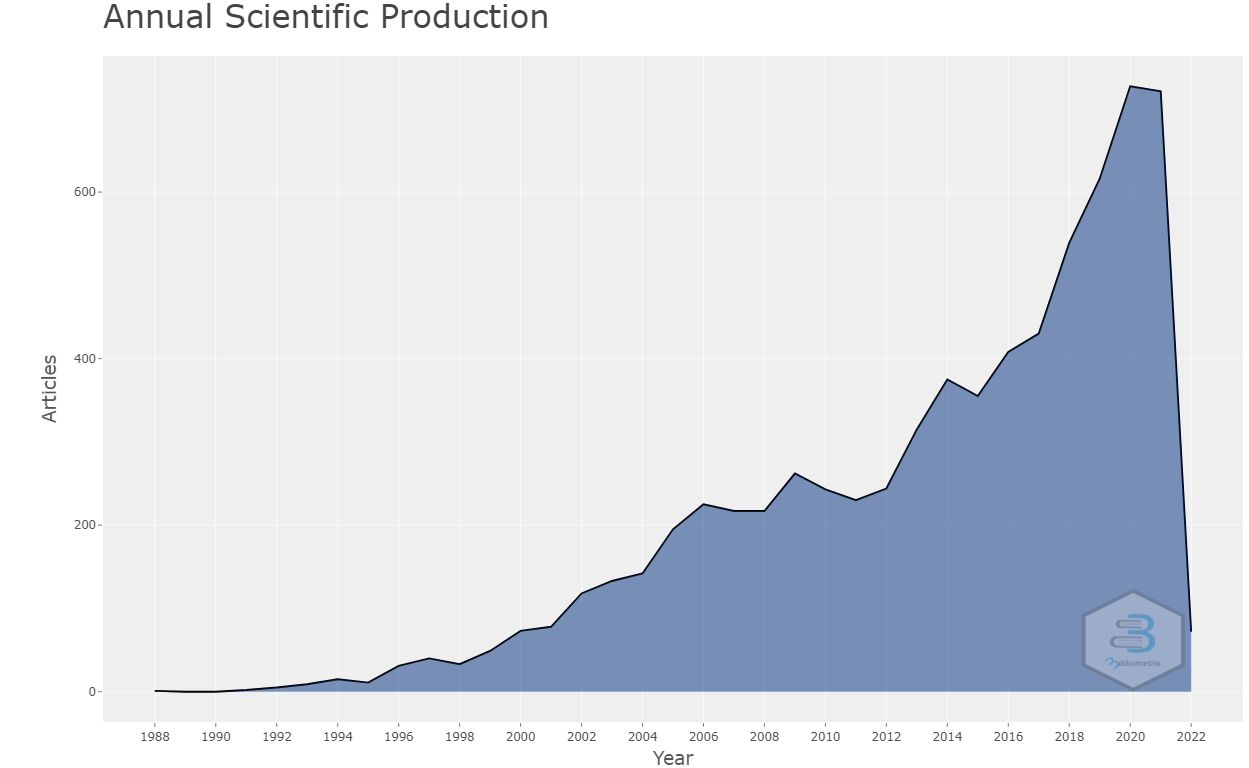
\includegraphics[width=1\textwidth]{experiments/andrelarrosacrypt/AnaliseBibliometrica/CriptografiaQuantica/imagens/CQA@andrelarrosacrypt_ProdAnual.png}
    \caption{Evolução da produção científica no \dataset\ CQA@andrelarrosacrypt.}
    \label{CQA@andrelarrosacrypt_ProdAnual}
\end{figure}

A figura \ref{CQA@andrelarrosacrypt_ProdAnual} representa a evolução da produção de documentos relacionados ao tema do \dataset\ CQA@andrelarrosacrypt, de 1988 até 2022. Como os dados foram coletados no início de 2022, a produção específica desse ano ainda é baixa, mas, como o gráfico segue uma curva aproximadamente exponencial, é de se esperar que acompanhe o nível de 2020 e 2021.



\subsection{Interpretação do Crescimento}

Como destacado na \href{https://www.quthought.com/post/history-of-quantum-computing-a-timeline}{Linha do Tempo}, o desenvolvimento da computação quântica nos anos 1990 é representado na figura como o início do crescimento das pequisas. Na mesma referência, percebemos que nos últimos dez anos empreses como Google e IB, além de instituições como NASA e NSA tem investido nesse assunto. Indicando, não só um interesse econômico, mas uma necessidade governamental.

Se considerarmos os interesses da NSA (Agência de Segurança Nacional dos Estados Unidos), percebemos como esse novo tipo de computação está alterando a meneia como vemos codificação e decodificação de informações. 


\subsection{Evolução das Citações}

\begin{figure}
    \centering
    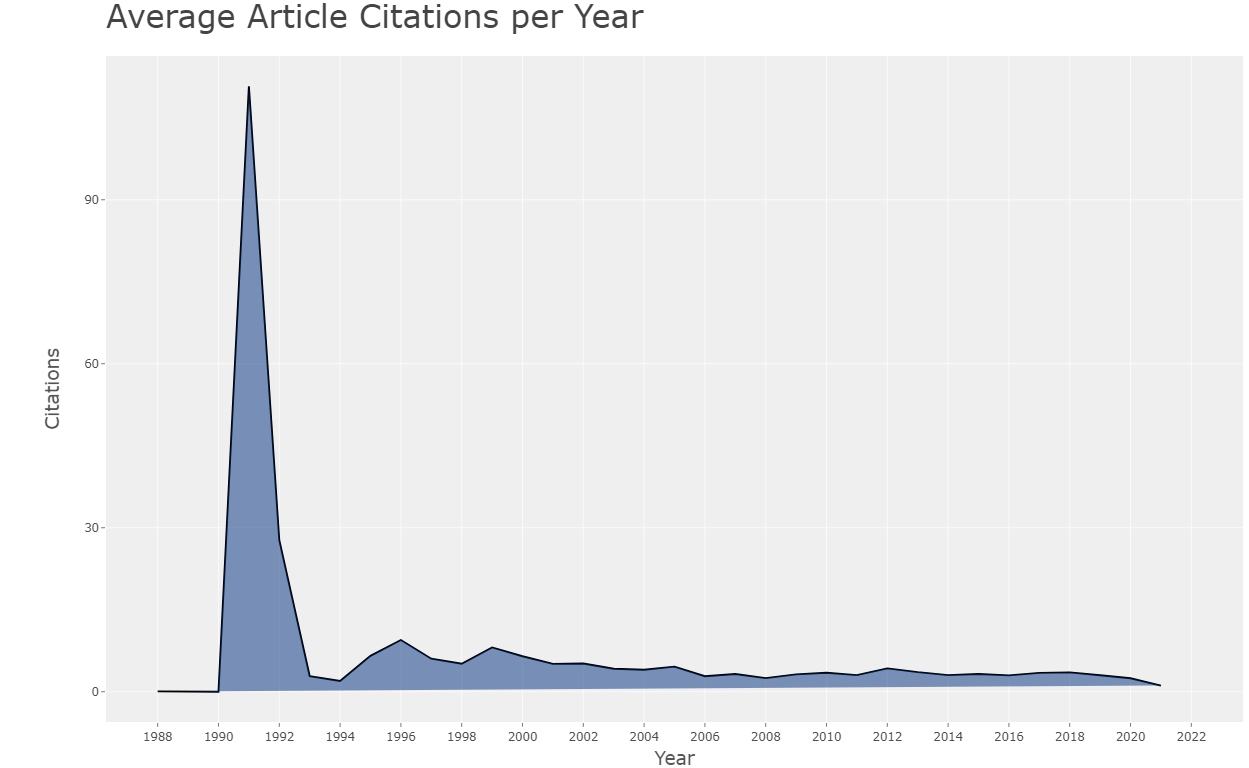
\includegraphics[width=1\textwidth]{experiments/andrelarrosacrypt/AnaliseBibliometrica/CriptografiaQuantica/imagens/CQA@andrelarrosacrypt_CitaAnual.png}
    \caption{Evolução das citações ao \dataset\ CQA@andrelarrosacrypt.}
    \label{CQA@andrelarrosacrypt_CitaAnual}
\end{figure}

No geral, o número de citações anuais se mantém estável ao longo dos anos, com uma média de aproximadamente 4. Contudo em 1991 o número de citações atingiu 110.8, provavelmente, isso ocorreu por coonta da publicação do artigo \textit{Quantum cryptography based on Bell’s theorem} que recebeu um total de 6852 citações.

\subsection{Interpretação das Citações}

Interessante mostrar que, embora haja uma grande crescimento na produção de documentos abordando o tema de Criptografia Quântica, como mostrado na figura \ref{CQA@andrelarrosacrypt_ProdAnual}, o número médio de citações não parece aumentar, figura \ref{CQA@andrelarrosacrypt_CitaAnual}. Talvez a explicação seja que os artigos mais relevantes são antigos, ou seja, os novos estudos não tão significativos.

\begin{figure}
    \centering
    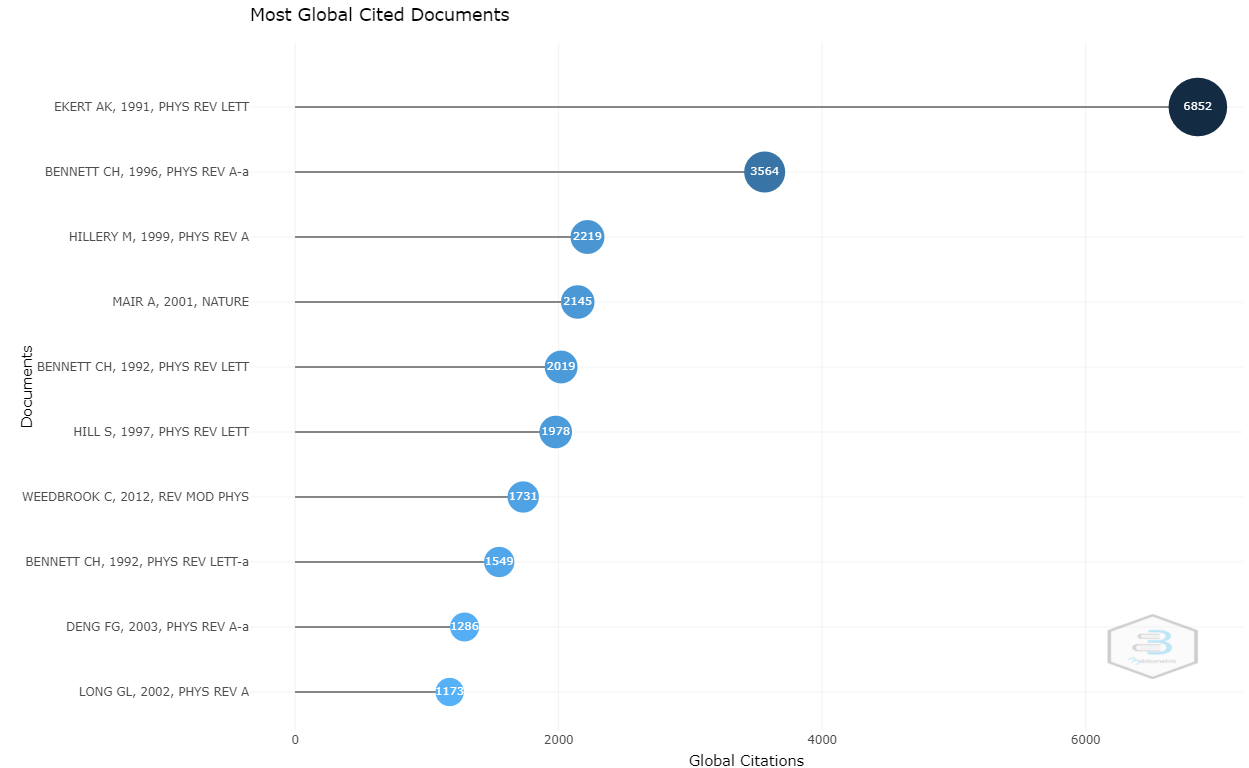
\includegraphics[width=1\textwidth]{experiments/andrelarrosacrypt/AnaliseBibliometrica/CriptografiaQuantica/imagens/CQA@andrelarrosacrypt_MostCit.png}
    \caption{Artigos mais citados do \dataset\ CQA@andrelarrosacrypt.}
    \label{CQA@andrelarrosacrypt_MostCit}
\end{figure}

Analisando a figura \ref{CQA@andrelarrosacrypt_MostCit} vemos que seis são dos anos 1990, três do início dos anos 2000 e um documento de 2012. O mais citado dessa lista é de 1991, o que parece solidificar a teoria de que os novos documentos não são tão relevantes. Se considerarmos que os novos documentos não tiveram tanto tempo para se popularizarem, poderíamos ter uma justificativa, mas a figura \ref{} contradiz essa explicação. Como vemos, com exceção dos trabalho de \textit{Weedbrook} de 2012 (que parece se tornar cada vez mais relevante), os novos documentos não aparentam estarem crescendo na comunidade científica. Portanto, é provavelmente que o conhecimento mais importante sobre o assunto, divulgado até agora, tenha sido publicado a pelo menos 20 anos.

\subsection{\textit{Three-Field Plots}}

Gráficos do tipo \textit{Three-Field Plots} exibem três campos (autores, documentos, referências, entre outros) e como eles se relacionam (\textit{Sankey Diagram}).

\subsubsection{\textit{Three-Field Plots} Autores, Referências e Palavras-chave}

\begin{figure}
    \centering
    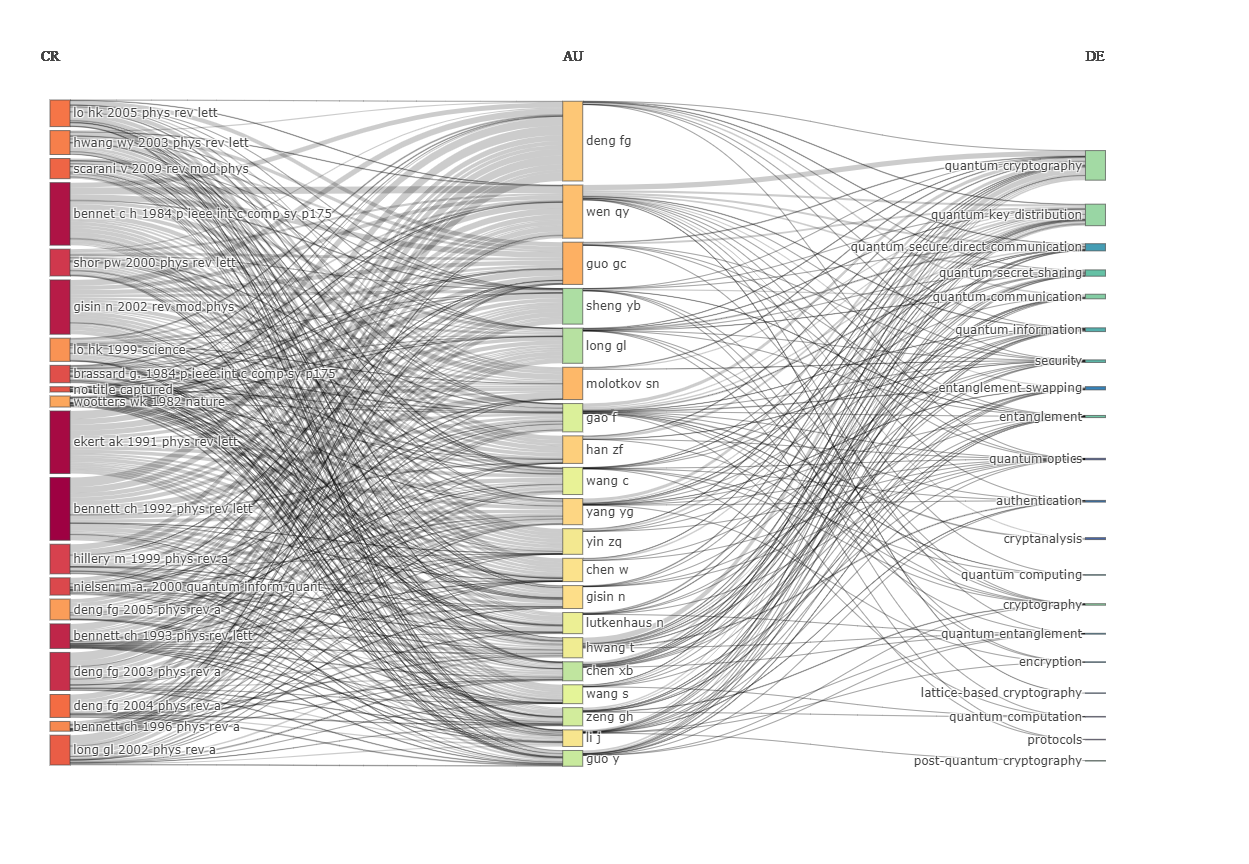
\includegraphics[angle=0,width=1\textwidth]{experiments/andrelarrosacrypt/AnaliseBibliometrica/CriptografiaQuantica/imagens/CQA@andrelarrosacrypt_Aut_Ref_Key.png}
    \caption{\textit{Three-Field Plots} do \dataset\ CQA@andrelarrosacrypt: 20 Autores, 20 Referências e 20 Palavras-Chave mais relevantes.}
    \label{CQA@andrelarrosacrypt_Aut_Ref_Key}
\end{figure}

A figura \ref{CQA@andrelarrosacrypt_Aut_Ref_Key} apresenta o gráfico \textit{Three-Field Plots} do  \dataset\ CQA@andrelarrosacrypt. Os campos de interesse destacados nesse gráfico são autores (centro), referência citadas (esquerda) e palavras-chave (direita) mais importantes.

No campo \textit{autores}, percebemos que 19 aparentam ser de origem asiática (mais provavelmente chinesa), o único não asiático provavelmente é russo (molotkov sn). Por outro lado, as referências apresentam maior heterogeneidade, com documentos aparentemente asiáticos, europeus e norte-americanos. Isso nos sugere que pesquisadores de origem chinesa tem migrado para países ocidentais ou tem trabalhado em direta colaboração com pesquisadores europeus e norte-americanos.

Relevante cometar que o autor mais destacado é \textbf{deng fg} e nas referências mais citadas temos três trabalhos de sua autoria \textbf{}{Deng FG, 2003, PHYS REV A} - DOI 10.1103/PhysRevA.68.042317 (protocolo para comunicação quântica segura), \textbf{Deng FG, 2004, PHYS REV A} - DOI 10.1103/PhysRevA.69.052319 (outro protocolo para comunicação quântica segura) e \textbf{Deng FG, 2005, PHYS REV A} - DOI 10.1103/PhysRevA.72.044302 (análise de protocolo de comunicação segura proposto por Zhang, Li, and Man). O que nos mostra a relevância de tal autor e seu aparente foco na área de comunicação segura.

Ao estudarmos as \textit{palavras-chaves} fica claro o focos desses autores no temos de comunicação quântica segura, \textbf{quantum secure direct communication}, \textbf{quantum secret sharing} e \textbf{quantum communication}, e o uso de criptografia quântica, \textbf{quantum cryptography} e \textbf{quantum key distribution}, para tal fim.


\subsubsection{\textit{Three-Field Plots} Autores, Afiliações e Países}

\begin{figure}
    \centering
    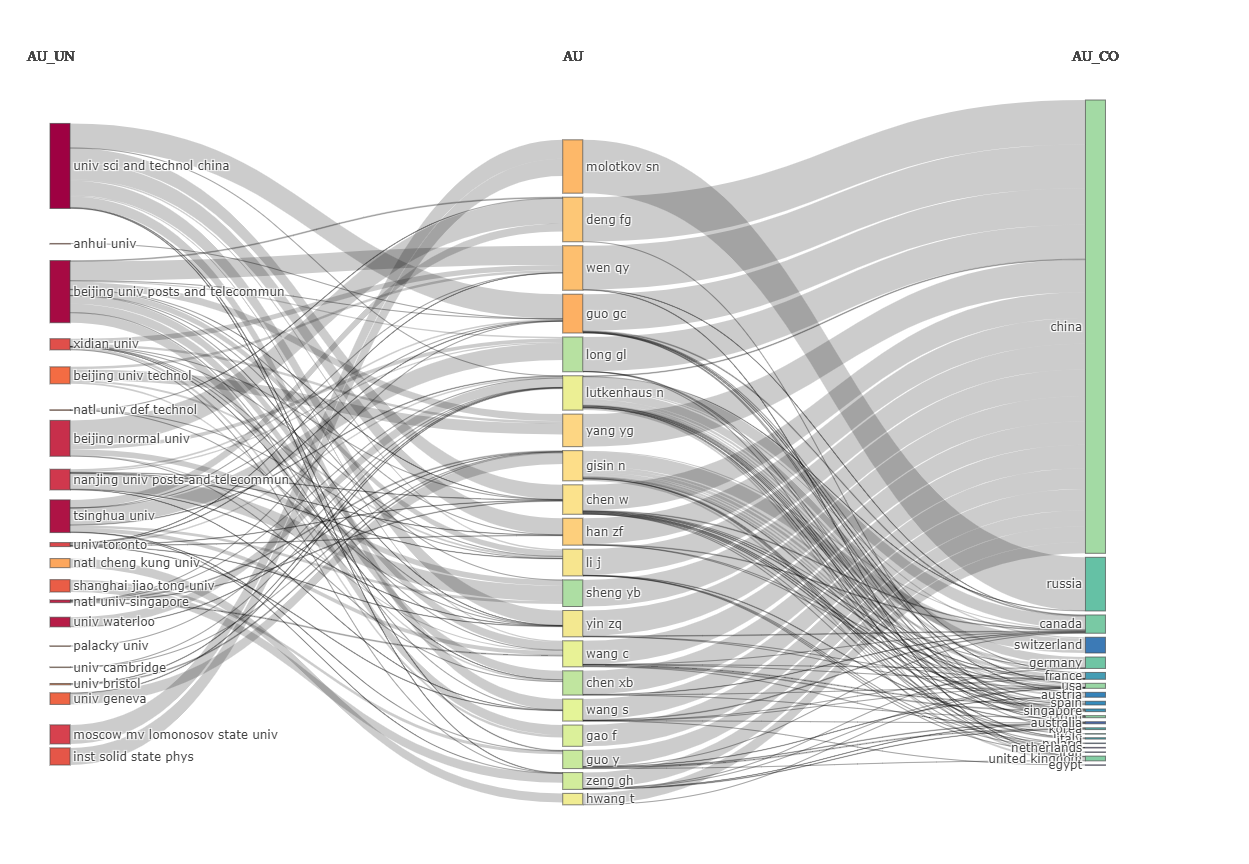
\includegraphics[angle=0,width=1\textwidth]{experiments/andrelarrosacrypt/AnaliseBibliometrica/CriptografiaQuantica/imagens/CQA@andrelarrosacrypt_Aut_Aff_Coun.png}
    \caption{\textit{Three-Field Plots} do \dataset\ CQA@andrelarrosacrypt: 20 Autores, 20 Instituições e 20 Países mais relevantes.}
    \label{CQA@andrelarrosacrypt_Aut_Aff_Coun}
\end{figure}


O gráfico da figura \ref{CQA@andrelarrosacrypt_Aut_Aff_Coun} confirma as suspeitas em relação à origem chinesas da maioria dos autores. Mesmo com a prevalência da China, temos a Rússia, Canada, Suíça, Alemanha, França e Estados Unidos com significativa influência.

Com relação às instituições afiliadas, notamos um predomínio das universidades chinesas, o que pode indicar que esses pesquisadores chineses estão trabalhando na China e não em universidades estrangeirais como havia sido sugerido. Observando o campo dos países, percebemos que muitos dos pesquisadores chineses tem afiliações com outros países. Isso indica que a segunda teoria apontada anteriormente, colaboração com pesquisadores ocidentais, parece ser verdade.

\section{Estrutura Conceitual}

\begin{figure}
    \centering
    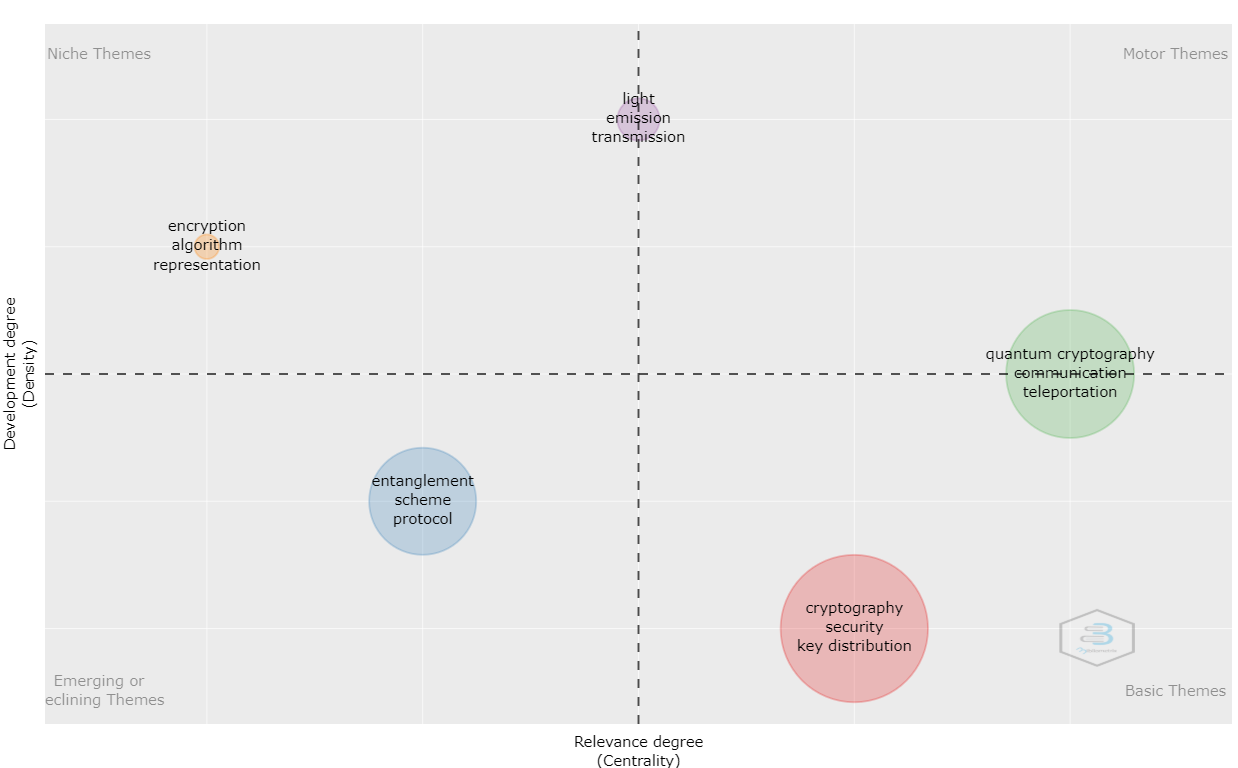
\includegraphics[angle=0,width=1\textwidth]{experiments/andrelarrosacrypt/AnaliseBibliometrica/CriptografiaQuantica/imagens/CQA@andrelarrosacrypt_MapaTematico.png}
    \caption{Mapa temático do \dataset\ CQA@andrelarrosacrypt.}
    \label{CQA@andrelarrosacrypt_MapaTematico}
\end{figure}

Fazendo um estudo da figura \ref{CQA@andrelarrosacrypt_MapaTematico} identificamos cinco aglomerados de conceitos que definem as principais áreas de estudo. Termos como \textbf{cryptograpy}, \textbf{quantum cryptograpy}, \textbf{entanglement}, \textbf{algorithm}  são esperados considerando o tema do nosso estudo. O que mais interessa são as expressões que, a priori, não parecem condizer com a pesquisa, essas que vamos focar.

Primeiro, temos em azul duas palavras que necessitam de explicação, \textbf{scheme} e \textbf{protocol}. Ambas fazem referência à comunicação segura e suas regras no mundo quântico. Passando para o aglomerado vermelho, encontramos \textbf{key distribution} está relacionado à um problema em criptografia que envolve a distribuição de chaves de acesso às partes interessadas, o que faz sentido considerando as demais expressões nesse mesmo aglomerado. Com relação ao agregado verde, temos \textbf{teleportation}. Ela se refere à teletransportação quântica, um método de se transferir informação quântica. Por fim, temos o bloco roxo, \textbf{light}, \textbf{emission} e \textbf{transmission}, todos apontam para as ótica quântica que estuda, dentre outras coisas, o uso de fótons de luz para transportar/processar informação.

\section{Estrutura Intelectual}

\begin{figure}
    \centering
    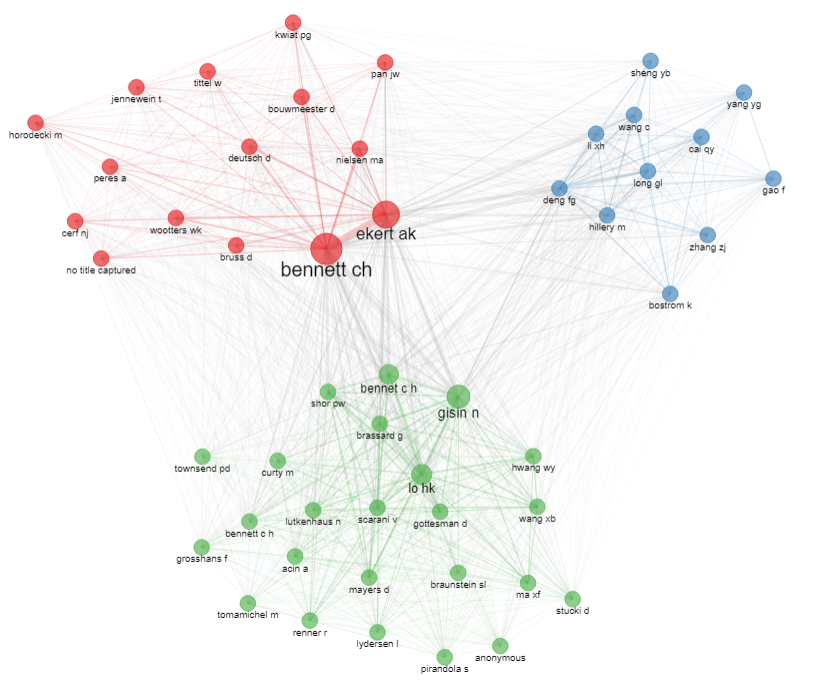
\includegraphics[angle=0,width=1\textwidth]{experiments/andrelarrosacrypt/AnaliseBibliometrica/CriptografiaQuantica/imagens/CQA@andrelarrosacrypt_CoCit.png}
    \caption{Rede de co-citação do \dataset\ CQA@andrelarrosacrypt.}
    \label{CQA@andrelarrosacrypt_CoCit}
\end{figure}

Com relação à estrutura intelectual visível na figura \ref{CQA@andrelarrosacrypt_CoCit}, temos três principais grupos. Em vermelho encontramos o que parecem ser autores ocidentais, em azul autores chineses e em verde autores ocidentais e chineses. Podemos esperar que os autores de cada grupo estejam trabalhando em temas semelhantes, pois citam os trabalhos um do outro.

O autor de maior influência no grupo vermelho é \textit{Bennett}. Seus dois artigos mais citados, ambos de 1992, \textit{Quantum cryptography using any two nonorthogonal states} e \textit{Quantum cryptography without Bell’s theorem}. Como podemos perceber, tratam de estratégia e técnicas de criptografia quântica. Podemos esperar que os autores que citam Bennett também desenvolvem desse assunto. Para confirmar nossas suspeitas, temos \textit{Ekert} e seu artigo \textit{Quantum cryptography based on Bell’s theorem}, que também aborda diretamente a questão da criptografia.

No aglomerado azul, todos parecem estar no mesmo nível, no que diz respeito à citações. Pegando como exemplo \textit{Deng}, seu artigo mais citado é \textit{Two-step quantum direct communication protocol using the Einstein-Podolsky-Rosen pair block}, que trata de protocolo de comunicação apoiado em aspectos da teoria quântica. Se selecionarmos outro autor do mesmo grupo, \textit{Li}, vemos que seu trabalho mais citado, \textit{Improving the security of secure direct communication based on the secret transmitting order of particles} também trata de comunicação. Logo, parece seguro afirmar que esse grupo foca em elemento de comunicação (segura) utilizando fatores da teoria quântica.

Por fim, no grupo verde, temos \textit{Lo} como influente autor. Seu trabalho mais citado localmente \textit{Unconditional Security of Quantum Key Distribution over Arbitrarily Long Distances} aborda comunicação segura (como o grupo azul) sob o ponto de vista de chave chave distribuída. Novamente, se observarmos o trabalho de \textit{Gisin}, \textit{Trojan-horse attacks on quantum-key-distribution systems}, vemos o mesmo tópico.


\section{Estrutura Social}

\begin{figure}
    \centering
    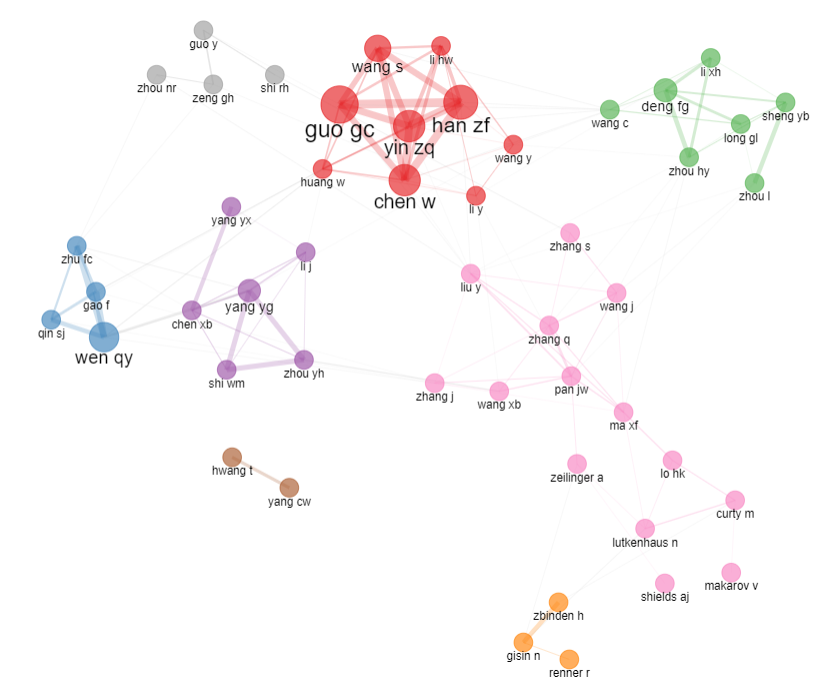
\includegraphics[angle=0,width=1\textwidth]{experiments/andrelarrosacrypt/AnaliseBibliometrica/CriptografiaQuantica/imagens/CQA@andrelarrosacrypt_Colab.png}
    \caption{Rede de colaboração do \dataset\ CQA@andrelarrosacrypt.}
    \label{CQA@andrelarrosacrypt_Colab}
\end{figure}

Na figura \ref{CQA@andrelarrosacrypt_Colab} vemos as colaborações entre autores. Os grupos parecem ser divididos em instituições, com exceção dos autores em rosa que são de instituições distintas. O grupo rosa parece correlacionar com as colaborações entre pesquisadores chineses e ocidentais descrita anteriormente.

\begin{figure}
    \centering
    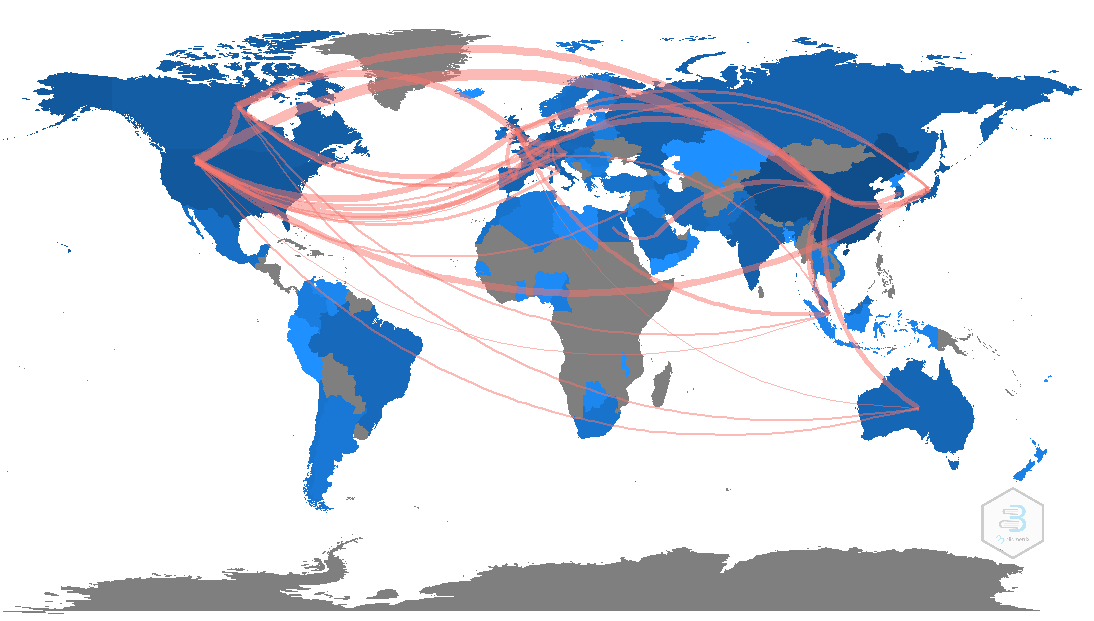
\includegraphics[angle=0,width=1\textwidth]{experiments/andrelarrosacrypt/AnaliseBibliometrica/CriptografiaQuantica/imagens/CQA@andrelarrosacrypt_ColabMap.png}
    \caption{Mapa de colaboração do \dataset\ CQA@andrelarrosacrypt.}
    \label{CQA@andrelarrosacrypt_ColabMap}
\end{figure}

Complementando as informações anteriores, na figura \ref{CQA@andrelarrosacrypt_ColabMap} evidencia as colaborações entre:

\begin{itemize}
    \item China - Estados Unidos
    \item China - Canada
    \item China - Alemanha
    \item China - Reino Unido
    \item Estados Unidos - Canada
    \item Estados Unidos - Reino Unido
\end{itemize}

Com enfase na relação Estados Unidos - China. Esses dados estão de acordo com o cenário geral de pesquisa científica, com norte-americanos e chineses dominando as áreas de conhecimento.